\PassOptionsToPackage{dvipsnames}{xcolor}
\documentclass[a4paper,11pt]{book}
\usepackage[]{geometry}

\usepackage{ucs}
\usepackage[utf8]{inputenc}
\usepackage{amsmath}
\usepackage{amssymb}
\usepackage{siunitx}
\usepackage{cancel}
\usepackage[italian]{babel}
\usepackage{fontenc}
\usepackage{graphicx}
\graphicspath{{img/}}
\usepackage{circuitikz}
\ctikzset{
    resistors/scale=0.7,
    capacitors/scale=0.7,
    inductors/scale=0.7,
    sources/scale=0.7
    }

\usepackage{float}
\usepackage{xcolor}

\usepackage{hyperref}
\hypersetup{
    colorlinks=true,
    linkcolor=black,
}
\usepackage{arydshln} % dashed lines in matrix (array)



%Definizione 'globale' larghezza immagini
\newcommand{\picwid}{0.35\linewidth}
\usepackage{tikz}
\usepackage{pgfplots} % Plot dei grafici
\pgfplotsset{compat=1.18}
% Riduzione tempi di compilazione esternalizzando le figure in pdf separati
\usepgfplotslibrary{external}
%\usetikzlibrary{pgfplots.external}
\tikzexternalize[prefix=tikz/, optimize command away=\includepdf]
\usetikzlibrary{patterns} % libreria per disegnare i pattern
%\tikzset{prefix={tikz/}}


\usepackage{caption}
\usepackage{subcaption}

\usepackage{polynom}

\newcommand{\Lap}{\ensuremath{\mathcal{L}}} %L di Laplace
\renewcommand{\Re}{\ensuremath{\mathfrak{Re}}} %Parte reale
\renewcommand{\Im}{\ensuremath{\mathfrak{Im}}} %Parte immaginaria

\usepackage{diagbox} %pacchetto linea diagonale per tabelle
\usepackage{booktabs} % toprule midrule e bottomrule
\usepackage{steinmetz} %pacchetto per notazione angolo

\usepackage{bodegraph} %pacchetto per diagrammi di Bode

\date{\today}
\title{Appunti Sistemi Energetici Innovativi}
\author{Daniele Olivieri}
\begin{document}
\maketitle
\tableofcontents
%Vedi il libro motori di Ferrari
\include{lezione_01}

\chapter{Introduzione allo studio delle Macchine a Fluido}

Le macchine a fluido si dividono in due grandi famiglie
\begin{itemize}
\item Dinamiche, come compressori e turbine, a flusso continuo

\item Volumetriche, come i motori a combustione interna o pompe e compressori,
il lavoro è svolto mediante una variazione di volume
\end{itemize}

Le macchine si suddividono ulteriormente in:
\begin{itemize}
\item Macchine motrici
\item Macchine operatrici
\end{itemize}
 e ancora in
\begin{itemize}
\item Macchine termiche (IMT)
\item Macchine idrauliche
\end{itemize}

Nelle macchine termiche è sempre presente un ciclo termodinamico, del calore
che riduce sempre i rendimenti, nelle macchine idrauliche invece, lavorando ``a
freddo'' l'energia restituita è quasi interamente pari a quella fornita dal
fluido.

Rispetto alla direzione del moto del fluido si parlerà di macchine
\begin{itemize}
\item Assiali
\item Radiali
\item A flusso misto
\end{itemize}

Mediante l'equazione di Eulero è possibile...

\section{Macchine termiche}
La macchina termica non è l'impianto termico,
Esempio con gruppo turbogas
%Inserisci immagine turbogas

Il generatore è posizionato solitamente vicino al compressore e non alla
turbina per le più basse temperature, a meno che la turbina non sia
multiassiale.

Il moto del fluido può essere stazionario come ad esempio in una turbina, il
flusso è continuo, in realtà è un'approssimazione; oppure in un flusso non
stazionario come in un motore a combustione interna.

Alcuni fluidi sono comprimibili o lo sono talmente poco da essere ritenuti
incomprimibili.

Un fluido può essere viscoso o non viscoso

Nel caso di grossi impianti le turbine possono essere simmetriche, disposte su
due lati come se fossero due turbine collegate.

Gli impianti motore termici possono essere
\begin{itemize}
 \item Impianti a vapore; 2MW - 1000MW
 \item Turbina a gas; 18kW - 500MW
 \item Motori a combustione interna; 0.1kW - 90MW
 \item Impianti combinati (gas-vapore); $>$ 1000MW
\end{itemize}

Le grandezze in ingresso sono calore (kW), in uscita potenza meccanica (kW).

Le turbine idrauliche hanno invece potenze medie superiori a 100MW.


Formula del rendimento di un ciclo combinato, alla potenza della turbina a gas
si aggiunge la potenza della turbina a vapore:
\begin{equation}
\eta_g = \frac{L_u}{m_c\cdot H_i} =\frac{P_u}{\dot{m}_c \cdot H_i} =
\frac{P+P_{TV}}{\dot{m}_f H_i}
\end{equation}

Si ricorda la definizione di portata massica
\begin{equation}
\dot{m}_c = \frac{dm_c}{dt}
\end{equation}

In passato le temperature massime erano limitate dai materiali della turbina,
non c'era abbastanza calore residuo per alimentare la turbina a vapore, per
questo motivo non si realizzavano cicli combinati.

Il rendimento di un impianto è spesso inferiore se l'impianto non lavora a
massima potenza.
Un ulteriore limite della turbina a gas è la temperatura di ingresso dell'aria,
può essere a volte comodo raffreddare inizialmente l'aria d'ingresso al
compressore.

In un gruppo turbogas, solitamente la turbina ha meno stadi, il compressore
deve eseguir un lavoro ``forzato'' contro la tendenza naturale dell'aria ad
espandere, sono necessari più stadi.
Nella turbina il gas espande, avverrebbe anche in maniera naturale, non è
dunque necessario un elevato numero di stadi.
%museo tecnico Spira germania

Rendimento di un impianto idraulico
\begin{equation}
 \eta_G = \frac{P}{\rho\cdot g \cdot h \cdot Q}
\end{equation}
$Q$ è la portata volumetrica, $\rho$ è la densità e $h$ è l'altezza geodetica.

L'energia prodotta in un impianto sarà l'integrale della potenza, oppure il
prodotto tra la potenza e il fattore di utilizzo $f$
\begin{equation}
 E_{kWh} = \int_0^T P_{\text{effettiva}} dt = f\cdot P_n \cdot T
\end{equation}

\section{Cicli termodinamici}
I cicli possono essere suddivisi in reali e ideali
VEDI TABELLA SLIDE

In un ciclo ideale si effettua una trasformazione isoentropica, ad entropia
costante, in caso contrario si sta riducendo energia meccanica, ovvero si
distrugge l'\textit{exergia}, con conseguente produzione di entropia.

Consumo specifico di calore
\begin{equation}
 C_s = \frac{1}{\eta_G} = \frac{m_c\cdot H_i}{L_u}
\end{equation}

VEDI SIDE CON I RENDIMENTI

Aggiungi rendimento di combustione

Per disegnare un ciclo termodinamico si rappresentano prima le due isobare
divergenti, poi si congiungono i punti con le trasformazioni, il calore di
adduzione, caratteristica del ciclo termodinamico, risente di tutto il ciclo e
 ne influisce il rendimento

Potere calorifico inferiore

Non si usa praticamente mai il potere calorifico superiore


Definizioni di DOSATURA
\begin{itemize}
 \item Rapporto aria / combustibile $ \alpha = \frac{m_a}{m_f}$
 \item Rapporto combustibile / aria $ f= \frac{m_f}{m_a} = \frac{1}{\alpha} $
 \item Rapporto di equivalenza $\varphi = \frac{f}{f_{st}} =
\frac{\alpha_{st}}{\alpha} \left\{
\begin{aligned}
>1\ & \text{Eccesso di combustibile}\\
=1\ & \text{Stechiometrico}\\
<1\ & \text{Eccesso di aria}
\end{aligned}\right.$
\end{itemize}

$\alpha_{st}$ è il rapporto aria / combustibile che si ottiene in caso di
reazione stechiometrica.

Nel calcolo delle masse è necessario inserire l'azoto nella massa d'aria che ha
un peso prevalente nella composizione dell'aria.

Quando si considera il metano come combustibile non bisognerebbe assumere il
metano come elemento singolo mentre il gas naturale realmente utilizzato è
solitamente composto al 90\% da metano e la restante parte da altri gas come
butano e propano.

Indice di emissione di CO2 pari al rapporto tra la massa di CO2 e la massa di
combustibile bruciata.

Oppure si può indicare l'indice di emissione moltiplicato per il consumo
specifico ottenendo i grammi di CO2 rispetto all'energia prodotta.
$$
EICO_{2f} = \frac{m_{CO2}}{m_f}1000 \Rightarrow EICO_{2W} = EICO_{2f}c_{sc}
$$

L'\textit{azoto} non partecipa attivamente alla combustione, non si ossida in
una reazione stechiometrica ma in caso di eccesso di ossigeno si ha comunque
una ossidazione parziale dell'azoto con il rilascio dunque di sostanze
inquinanti in atmosfera ($NO_x$).

\section{Equazione di stato dei gas}

$pV = nRT$

Classificazione dei sistemi termodinamici


Vedi definizione flusso stazionario slide, equazione di bilancio della massa
ecc

Nelle macchine alternative solitamente non è vero che il flusso e la portata
siano costanti in ogni istante del ciclo.

Ricorda che calore e lavoro non sono differenziali esatti!





\section{Richiami di termodinamica}

Nel caso di flusso incomprimibile si può avere un condotto a sezione variabile
per variare la velocità del flusso si possono usare condotti acceleranti
(ugelli) o deceleranti (diffusori).

Rallentando l'acqua in uscita dalla turbina si recupera l'energia cinetica
residua del flusso.

Il condotto è qualsiasi sezione di passaggio del fluido, non necessariamente un
``tubo'', come ad esempio lo spazio tra le palette della turbina.

In un motore a 4 tempi si ha una condizione di ``incrocio'' in cui entrambe le
valvole sono aperte.

Il lavoro è ritenuto positivo quando ``esce'' dal sistema mentre è negativo
quando il lavoro sulla macchina viene eseguito al sistema.

\subsection{Trasformazione reversibile}
Si parla di trasformazione reversibile se non si ha variazione di entropia,
ossia se non rimane alcuna traccia della trasformazione.
Se c'è produzione entropica stai degradando il lavoro.

Rendimento politropico(?)

$$
h = q+pv
$$

Sistemi chiusi, il lavoro è funzione della variazione di volume $pdv$
\begin{equation}
u_B - u_A = Q - L = \int_{s_A}^{s_B} Tds - \int_{v_A}^{v_B}pdv
\end{equation}

Sistemi aperti, il lavoro è funzione della variazione di pressione $vdp$
\begin{equation}
h_B - h_A = Q - L =  \int_{s_A}^{s_B} Tds + \int_{p_A}^{p_B} vdp
\end{equation}

In un compressore ad esempio si ha l'area sottesa al piano h-s il lavoro
d'attrito, nella parte superiore invece il lavoro di controrecupero.

\begin{figure}[h]
\centering
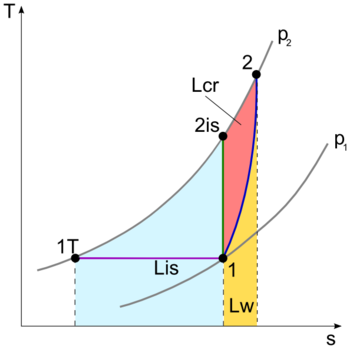
\includegraphics[width=0.4\linewidth]{compressione}
\end{figure}

Si parla di piano termodinamico del lavoro quello P-v,

Uno scambiatore di calore non prevede lavoro meccanico, non ha parti in
movimento..
Il termine $vdp$ si annulla a causa della pressione costante, quindi non c'è
lavoro mentre l'integrale $TdS$ mostra il lavoro fornito.
Innalzando la temperatura media di adduzione e sottrazione del ciclo si aumenta
il rendimento di Carnot.
$$
\eta_g = \eta_c\eta_r\eta_mm
$$
il termine critico è il rendimento reale $\eta_r$, il ciclo combinato è quello
con strategia per aumentare il pi¡u possibile le differenze di temperatura.

Solo per i \textit{processi reversibili} si ha l'uguaglianza tra l'incremento
di entropia e il prodotto $dQ$ e $1/T$, considerando una temperatura media
infatti
$$
s_B - s_A = \frac{\int_A^B \delta Q}{T_m} = \frac{Q}{t_m}
$$
Rendimento di Carnot:
\begin{equation}
\eta = \frac{Q_1-Q_2}{Q_1} = ... = 1 - \frac{T_{ms}}{T_ma}
\end{equation}


Al limite si desidera un rendimento unitario.

\subsection{Cause di irreversibilità}
SI prenda in esempio uno scambiatore a flussi
sparati.
Ci sarà sempre un limmite di ingombro, dunque non tutto il calore può passare
del fulolso caldo e non per lo scambiatore caldo.
La produzione entropica aumenta all'aumentare delle distanze tra le
temperature.
Non si superano di solito gli 8 spilllamenti per gli scambiato fa vatto.

Lavoro di attrito
In un condotto si ail...


In un impianto a vapore si ha una sottrazione di calore a temperatura costante
e a d un valore di calroad'acqua staavvenend.
%Inserisci foto ciclo HIRN
L'adduzione del calore avviene ad una temperatura relativamente bassa.

La caldaia a vapore è composta in tre parti
Economizzatore, vaporizzatore, surriscaldatore.

Spillando vapore dalla turbina psi piö otitmizzare la temperature in ingresso,
ovvero avere acqua in ingresso al generatore di vapore con una teoirad iche tii.

La potenza in un impianto vapore si scrive con
$$
P = \dot{m}_{VAP}\cdot\Delta h\cdot\eta_{m}
$$

Il salto entalpico è quello che massimizza il rendimento.



Nella realtà non c'è mai una trasformazione isobara in camera di combustione,
esistono delle piccole cadute di pressione in camera di combustione.

Con la rigenerazione si spilla vapore dalla turbina, cambia l'integrale Tds del
ciclo, partendo da una temperatura iniziale più alta si risparmia calore,
ovvero si risparmia combustibile, pari a
$$
\Delta Q_1 = \eta_b\Delta \dot{m}_f H_i
$$

Gli spillamenti non possono mai essere completamente chiusi, la turbina è
costruire per possedere una certa quantità di spillamenti, è disegnata per
contenere una certa portata d'acqua, si può sostituire lo scambiatore di
recupero con un impianto solare ad esempio.


La generazione entropica in uno scambiatore è legata alle differenze di
temperature per il lorop prodotto.
La produzione entropica distrugge l'exergia.

Vanno inseriti più spillamenti e più scambiatori di calore per ridurre le
irreversibilità.




\section{I cicli della turbina a gas}
L'impianto turbogas è composto da tre componenti, compressore, camera di
combustione e turbina, può essere presente un circuito di recupero dell'aria.

Tutte le grosse macchine sono di tipo assiale multistadio, è un impianto molto
flessibile, può lavorare con molte tipologie di combustibili diversi.

Le turbine possono essere monoalbero o multialbero, la seconda configurazione
permette al generatore elettrico di mantenere la sua velocità imposta dalla
frequenza di rete senza rischiare di far stallare il compressore.
Nonostante le rappresentazioni grafiche il generatore è in realtà collegato al
compressore e non alla turbina a causa delle più basse temperature.

Il ciclo è il ciclo termodinamico, il circuito rappresenta come è costruito
l'impianto.
Alcuni impianti a circuito chiuso possono utilizzare l'elio anziché l'aria.
Il compressore va regolarmente lavato, sia durante il funzionamento che durante
manutenzioni straordinarie, questo per preservare le prestazioni dell'impianto.

I lavori specifici di un impianto turbogas sono comunque solitamente molto
bassi con l'aria, per questo può essere comodo cambiare il fluido dell'impianto
ed utilizzare ad esempio l'elio. Il compressore ad esempio assorbe gran parte
del lavoro prodotto dalla turbina, rispetto ad una pompa presente in un
impianto a vapore, utilizzando l'interrefrigerazione è possibile ridurre il
lavoro del compressore.


\subsection{Grandezze caratteristiche}
\begin{itemize}
 \item Rapporto di compressione $\beta = \frac{p_2}{p_1} = \frac{p_3}{p_4}$
 \item Rapporti di temperature $\theta = \frac{T_3}{T_1}$ rapporto tra la
massima e minima temperatura
\end{itemize}
Se si considera un ciclo ideale si può utilizzare l'equazione di stato dei gas
$$
\frac{p}{\rho} = RT
$$

Se il gas è ideale i calori specifici sono costanti, dipendono da $R$ e $k$,
$k=\frac{c_p}{c_v}$ è l'esponente dell'adiabatica, dipende dal gas in uso,
mentre $R=c_p-c_v$

Per il calcolo del salto entalpico si usa la seguente relazione
$$
\Delta h = Q - L = cp\Delta T
$$


Il ciclo ideale è quello di riferimento, tutte le trasformazioni adiabatiche
sono legate da
$$
\frac{dp}{dv} = -j \frac{v}{?}
$$

%Inserisci il lavoro di compressione.
$$
|L_C|= d\int_1^2 VDP = \frac{k}{k-1}1V_1(\beta^\lambda
-1)
$$

L'adduzione del calore durante la combustione invece
$$
L_t = \int_3^4 = \frac{k}{k-1z}p_3v
$$

La temperatura media di un impianto turbogas è relativamente alta mentre la
temperatura di sottrazione non è facilmente modificabile, dipende dalla
temperatura ambiente ma dipende dalla temperatura di scarico dei gas combusti,
solitamente anche a $500^\circ$


Il lavoro utile è dato dalla differenza tra il lavoro prodotto dalla turbina e
quello assorbito dal compressore.

Il rendimento è funzione solo di $\beta$ nel ciclo ideale, solitamente però il
rapporto $\beta$ dipende dal tipo di applicazione.

Se si usa un impianto a circuito chiuso con elio si massimizza il lavoro con
una macchina più piccola, con rapporto di compressione inferiore.

Il $C_p$ dell'aria è solitamente circa 1, in realtà per la turbina il $C_p$ dei
gas esausti è solitamente maggiore.



Per capire se una macchina è di grossa potenza si capisce dalla camera di
combustione, se fosse una turbina aeronautica dovrebbe essere a sezione
inferiore, il combustore si dice interno, altrimenti con combustore ad anello
la turbina non può essere aeronautica.

\section{Rigenerazione}
La turbina ha un lavoro utile relativamente basso a causa della potenza
necessaria a muovere il compressore.

Si innalza la pressione allo scarico della turbina se si aggiunge il
rigeneratore, si parla di contropressione allo scarico, dunque l'espansione
avviene in un salto entalpico inferiore, dunque si riduce leggermente la
potenza alla turbina. In impianti più complessi gli scambiatori possono essere
molteplici.
La temperatura del flusso in uscita è ancora rilevante, viene sfruttata per
riscaldare l'aria in uscita dal compressore, preriscaldando il flusso prima
della camera di combustione, dunque si risparmia combustibile, ovvero la Q_1 di
adduzione del calore.

Rendimento con rigenerazione, se la temperatura allo scarico della turbina è
molto più alta di quella dello scarico del compressore si può avere
interrefrigerazione.
Il rapporto $\beta$ massimo che massimizza il lavoro è pari a quello che si
otterrebbe con le temperatura $T2=T4$.

L'area sottesa alla curva $4r-r$ rappresenta il calore fornito dai gas caldi al
gas in camera combustione,
$Q_1=C_p(T_3-T_{2R})$
La temperatura di adduzione inoltre è aumentata.



Riducendo Beta (riducendo la taglia della turbina) invece si aumenta la
temperatura,

$$
\eta_d = 1- \frac{1}{\beta^\lambda}
$$


Calore recuperato
$$
|Q_{2r}| = C_p(T_4-T_r)
$$


Rendimento ideale del ciclo con rigenerazione:
$$
\eta_{id} \frac{L}{(Q_1)}
$$

Ha senso fare la rigenerazione con valori di $\beta$ piccoli, quindi macchine
piccole, va calcolato il $\beta$ massimo che massimizza il lavoro, se il
rapporto fosse superiore a questo valore si evita la rigenerazione.



\section{Interrefrigerazione}
Si utilizza questa tecnica per ridurre il lavoro specifico assorbito dal
compressore, spezzando la compressione tra macchine successive.
Viene chiamato anche intercooler lo scambiatore posto tra i due compressori,
viene utilizzato un fluido esterno come l'acqua per raffreddare l'aria un
uscita dal primo compressore.

Con l'interrefrigerazione si è ridotto il lavoro richiesto per la compressione,
il rendimento però è peggiorato, è necessario fornire più calore per riscaldare
il fluido fino al punto 3, per questo motivo può essere utile utilizzare la
rigenerazione e recuperare il calore della turbina per aumentare il rendimento,
il punto 2 infatti si trova ora molto più in basso rispetto al punto 4.

Nel ciclo reale, il ciclo aggiuntivo dovuto all'interrefrigerazione è uno
pseudo ciclo, ha la curva di raffreddamento ad entropia negativa, aumenta
dunque il rendimento, è come se fosse un ciclo ideale deformato.




\section{Cicli misti combinati}

Si consideri un impianto turbo gas, a questo viene collegato un impianto a
vapore al fine di migliorare i rendimenti.
%LIBRO LOZZA turbine a gas e cicli combinati

\subsection{Ciclo STIG}
Si aggiunge una caldaia in coda alla turbina nella quale circola dell'acqua che
vaporizza e successivamente entra in camera di combustione, riducendo le
temperature di picco riducendo la formazione di ossidi di azoto, immettono
inoltre nell'impianto una portata aggiuntiva, aumentando la potenza.

Al variare dei parametri fluidodinamici all'interno dell'impianto si avranno
delle variazioni dei punti di equilibrio, la prima macchina a notare la
variazione di portata è la turbina, in coda alla camera di combustione.
La pressione in ingresso alla turbina aumenta, aumentando leggermente il
rapporto di compressione $\beta$ si avvicina il compressore alla linea di
stallo fornita dal costruttore, dunque l'intero impianto va verificato.

In assetto cogenerativo si produce acqua calda ``sanitaria'', il vapore può
essere inviato sia in camera di combustione che all'utenza termica. Ad esempio
in inverno il compressore richiede meno potenza ??

Questa modifica viene sempre effettuata su una turbina bi-albero, al fine di
mantenere il numero di giri corretto al generatore, senza alterare le
prestazioni del ciclo termodinamico.

Questi cicli richiedono però un consumo d'acqua pari a 1-2 kg/Kwh, può essere
iniettata in quattro punti differenti, al fine di produrre cogenerazione,
oppure a monte della camera di combustione, all'interno della camera di
combustione oppure direttamente nella turbina di potenza (bassa pressione).

Approach point: differenza tra la temperatura del vapore acqueo in uscita dalla
caldaia e la temperatura del gas in ingresso.
Pinch point: punto di minima distanza tra la temperatura dell'acqua e dei gas
caldi, solitamente al termine del riscaldamento dell'acqua liquida, all'inizio
del cambio di fase che avviene a temperatura costante, sotto la curva a campana
dell'acqua.

Le macchine rotanti possono essere scalate al fine di variare le potenze senza
cambiare il progetto delle macchine, utilizzando la teoria della similitudine;
questa operazione non è possibile per la camera di combustione che invece deve
rispettare la lunghezza caratteristica legata la tempo di residenza della
combustione, funzione soltanto della reazione chimica.


\section{Ciclo ad iniezione d'acqua}
Si considera un impianto di base di tipo ``ICR'' InterCooledRefrigerated, si
rende più efficace o più ``spinta'' sia l'interrefrigerazione che la
rigenerazione, il loro limite era lo scambio termico, iniettando acqua al
circuito di interrefrigerazione e rigenerazione si ottiene un vapore con più
energia da miscelare con l'aria in uscita dal compressore per entrare poi in
camera di combustione.





% \include{lezione_07}
% \include{lezione_08}
% \include{lezione_09}
% \include{lezione_10}
% \include{lezione_11}
% \include{lezione_12}
% \include{lezione_13}
% \include{lezione_14}
% \include{lezione_15}
% \include{lezione_16}
% \include{lezione_17}
% \include{lezione_18}
% \include{lezione_19}
% \include{lezione_20}
% \include{lezione_21}
% \include{lezione_22}
% \include{lezione_23}
% \include{lezione_24}
% \include{lezione_25}
\end{document}
